%%%%%%%%%%%%%%%%%%%%%%%%%%%%%%%%%%%%%%%%%%%%%%%%%%%%%%%%%%%%%%%%%%%%%%%%%%%%%%%%
%2345678901234567890123456789012345678901234567890123456789012345678901234567890
%        1         2         3         4         5         6         7         8

\documentclass[letterpaper, 10 pt, conference]{ieeeconf}  % Comment this line out
\IEEEoverridecommandlockouts


\usepackage[ngerman]{babel}
\usepackage{paralist, tabularx}
\usepackage{subfigure}
\usepackage{amsmath}

\usepackage{soul}
\usepackage{xcolor}
\newcommand\sichen[1]{\textcolor{red}{sichen: #1}}
\newcommand\siqi[1]{\textcolor{blue}{siqi: #1}}
\title{\LARGE \bf
Data Plane Verification as Program Verification
}


\author{Siqi Liu,
Sichen Song
}

\usepackage[T1]{fontenc}
\usepackage{graphicx}
\usepackage{listings}
\begin{document}



\maketitle
\thispagestyle{empty}
\pagestyle{empty}



\section{INTRODUCTION}
Data plane verification is an emerging field of computer networking, in which the behavior of network data plane is verified to follow a specification. 

To perform data plane verification, the network topology and forwarder configurations are typically encoded into a model, which is checked against the specification. For example, the Header Space Analysis (HSA) encodes the network nodes into functions on packet state, which consists of packet header and packet location~\cite{hsa}. HSA then simulates a symbolic packet being forwarded through the network model to verify reachability and other properties. Anteater, on the other hand, models the network and its specification as SAT formulas on the packet header and reduces the network verification problem into a SAT problem, which can be solved using existing SAT solvers such as Z3~\cite{z3}.

The existing works focuses on verifying stateless network nodes and consequently does not work on networks with stateful load balancers or NAT boxes. Although data plane specification language has been proposed in NoD~\cite{nod} and NetPlumber~\cite{netp}, the languages has limited expressiveness and requires times for network operators to learn. Lastly, the generated model is hard to understand or debug due to extensive use of logical formulas.

To address the above issues, we investigation into modeling the data plane as a computer program and utilizing existing symbolic execution tool, KLEE~\cite{klee}, to verify network properties. In the following sections, we provide the feasibility of reducing network verification into a program verification in \S~\ref{sec:feasibility}. We then present the architecture of our verifier that reduce network verification into program verification in \S ~\ref{sec:overall}. We dive into details of code generation in \S~\ref{sec:codegen}. We also propose potential optimizations that could potentially use pre-computation to improve the performance of verification in \S~\ref{sec:opt}. Lastly we discuss the evaluation results in \S~\ref{sec:eval}.

The verification tool code is available at https://github.com/shsssc/stateful_network_verify.

\section{Feasibility Analysis}\label{sec:feasibility}

Symbolic execution for program verification models program input as a set of potential values and explores the control flow graph of the program by executing the program and adding path constrains to the symbolic variables whenever having conditional statements. By keeping track of a set of potential input that leads to certain execution path, feasibility of  execution path can be calculated by checking whether the path conditions is satisfiable. In this way, by exploring all reachable execution paths, the program can be verified.

Symbolic execution is similar to Header Space Analysis(HSA) as they both use equivalence classes of input to ensure efficient and comprehensive exploration a directed graph. Both of them also reason about reachability in the graph by transforming the problem as a satisfiability problem of path condition.

This similarity motivates us to explore the idea of transforming the network verification problem into a program verification problem and transform network reachability and other properties to verify into code reachability. 
The idea can be implemented by generating the network configuration and verification problem into a network simulator on symbolic packet inputs. This reduction can have the following advantages:

\begin{enumerate}
  \item The generated model is a network simulator written in C++, which is easier to understand and debug compared to logical formula based modeling.
  \item Existing optimizer in compiler such as constant propagation and dead code elimination can operate on the generated code.
  \item Stateful nodes such as NAT can be modeled as a mutable objects that forward packets.
  \item The specification is essentially C++ code operating on packet state or path, which is easier to learn by network operators.
  \item The generated network simulator can be executed with concrete packet input, which can be reused to debug network configurations by visualizing packet forwarding.
\end{enumerate}

However, verifying data plane relying on program verification has the following disadvantages:

\begin{enumerate}
 \item Existing program verification tools are used as black boxes. Consequently there's less chance to apply domain knowledge to fine tune the implementation details for performance optimization.
 \item Program verification solves path constrains with SMT solver such as Z3, which only gives a single example for each property violation.
\end{enumerate}

\section{Overall Design}\label{sec:overall}
The overall design of our network verification framework is illustrated in fig.~\ref{fig:arch}. 

To reduce data plane verification into program verification, code generation is extensively used. 
Code generator is the primary part of reducing data plane verification into program verification. 
The generators will generate a executable C++ program that asserts the property-to-verify with symbolic packet inputs such that symbolic execution can later be used to check these assertions. 
The output C++ code is also annotated with generated comments serving as hints to help the poster processor to translate code coverage report from KLEE into network verification results.

These generated C++ code will be compiled into LLVM intermediate representation (IR) using the LLVM C++ front end Clang++. 
These IR is then used by KLEE for symbolic execution. KLEE will invoke LLVM optimization passes on the input IR and symbolically execute the program to maximize line coverage and check if it can fail any assertion in the program. 
The resulting coverage file is then fed into a post processing script to check if the property-to-verify is maintained by the network. 
The generated comments by code generators acts has hints for the post processor to better understand the coverage and thus make verification decisions.

\begin{figure}[]
  \centering
  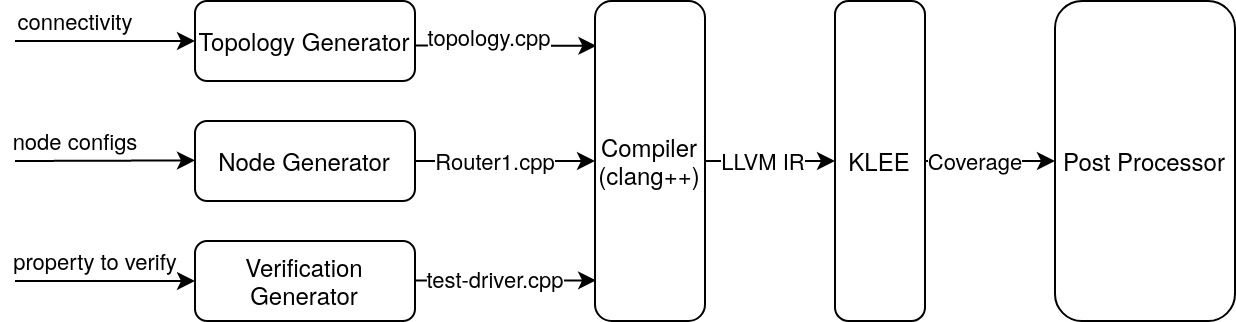
\includegraphics[width=\linewidth]{overview.png}
  \caption{Architecture}
  \label{fig:arch}
\end{figure}

\section{Code Generation}\label{sec:codegen}

Overall there are three different types of code generators: the network node generator, the topology generator, and verification generator. 
Network node generator generates forwarders and other nodes in the network from its configurations such as FIBs and ACLs. 
A variety of node types is supported such as ECMP routers and stateful NAT boxes. 
Topology generator generates the code that takes a packet state (header, location) as input and move a packet through the network for one step. 
The packet is first fed into the corresponding forwarder to make a forwarding action. 
The output packet is then transformed into a input packet of the next hop by looking up the network topology. 
Lastly, the verification generator will generate the "main function" that injects symbolic packets into the network and keep forwarding it through the network. 
The most import part of it is the main loop that keeps forwarding packets step by step using the topology generator. 
Depending on the property to verify, the generator may also record of packet paths and other states for later property checks. 
The code generators may embed comments in the generated code to facilitate post-processing.

The code generator are written with Python, and they uses jinja template library to insert required config parameter to the code template. 
These code generator are designed as modular classes, so that the operator can use a single script to invoke node, topology and verification generator for corresponding config information, and complete the verification. 

\subsection{Constrains}
Symbolic execution can perform poorly when the program has large loops, requires variable length in-memory data structures, or make many unnecessary branches. 
Being aware of these limitations, code generator of this framework inlines table (for example, FIB) lookup as a sequence of branches, instead of relying on in-memory data structures. 
It also bounds hop limit to bound the total amount of execution paths. 

\subsection{Packet State}
Inspired by HSA~\cite{hsa}, the packet state is the combination of header and location as shown in listing \ref{code:state}.
\begin{lstlisting}[language=C,caption=Packet State,label=code:state,captionpos=b]
struct Header {
  uint32_t src_address;
  uint32_t dst_address;
...
};

struct PktState {
  Header header;
  int node;
  int port;
};
\end{lstlisting}

\subsection{Stateless Network Routers}
Stateless network Routers are generated based on their FIB and ACL configurations. An C++ class with the node name is generated that has a \emph{forward} method that transforms the input packet state to the output packet state. Listing~\ref{code:stateless-router} shows a generated router class. Note that a linear scan over the routing table from longest prefix to shortest prefix is used for FIB lookup, which may result in poor performance. Optimization of FIB lookup is discussed in sec.~\ref{sec:opt}. Also, the \emph{[reached] Router4} comment act as a hint to facilitate post processing of node reachability.

\begin{lstlisting}[
  language=C,
  caption=packet state,
  label=code:stateless-router,
  captionpos=b,
  basicstyle=\small]
class Router4 {
  public:
  
  PktState 
  forward(PktState stateIn) { //[reached] Router4
    int node = stateIn.node;
    int portIn = stateIn.port;
    Header &header = stateIn.header;
    int portOut = forwardTable(header.dst_address);
    if (!acl(header, portIn, portOut)) 
        return {header, node, -1};
    return {header, node, portOut};
  }
  
  int forwardTable(uint32_t dst) {
  if ((dst >> 16) == (0xa000000 >> 16))//10.0.0.0/16
    return 1;
  if ((dst >> 16) == (0xa010000 >> 16))//10.1.0.0/16
    return 2;
  return -1;
    ...
  }
  
  bool acl(Header header, int ingress, int egress) {
    if (
    header.dst_port == 80 &&
    header.protocol == 6 &&
    true)
      return false; // DenyHTTP
    ...
    return true; // false as drop
  }
};
\end{lstlisting}


\subsection{Network}

The network with connectivity and node is generated as a C++ class, which instantiates all the nodes and expose a function that takes a packet state and makes one step of packet forwarding. The input packet is first processed by the corresponding forwarder to be transformed to an output packet. Then, by looking up network connectivity, the output packet is moved to the input port of the other end of the link.  Listing~\ref{code:topology} shows a generated network class.

\begin{lstlisting}[  language=C,
  caption=generated network class,
  label=code:topology,
  captionpos=b,
  basicstyle=\small]
class Topology {
  public:
  
  PktState 
  node_execute(PktState pktState) {
    int node = pktState.node;
    Header &header = pktState.header;
    int port = pktState.port;
    if (node == 0) {
      return node0.forward(pktState);
    }
    ...
    
    assert(0); //[node-dispatch-failed]
  }
  
  static PktState 
  link_function(PktState in) {
    int node = in.node;
    int port = in.port;
    Header &header = in.header;
    if (node == 0 && port == 1)
    return {header, 1, 1};
    if (node == 1 && port == 1)
    return {header, 0, 1};
    ...
  }
  
  public:
  Router1 node0;
  Router2 node1;
...
};
\end{lstlisting}

\subsection{Reachability Query Test Driver}
The reachability query test driver simply injects a symbolic packet at the user-selected node and simulate the packet forwarding until the packet exits or TTL runs out. KLEE will enumerate the entire header space trying to cover every line of code, which includes the forward method of each node object. Thus, the coverage report of KLEE can be used to infer if a node is reachable by checking if its corresponding class and method is covered. To cover a reasonable number of packet forwarding while bounding the main loop for packet forwarding, we set the TTL to be two times the diameter of the network topology.
Listing~\ref{code:reachability-driver} shows a generated reachability test driver.

\begin{lstlisting}[  language=C,
  caption=generated reachability/loop test driver,
  label=code:reachability-driver,
  captionpos=b,
  basicstyle=\small]
class Network : public Topology {
  public:
  void forward(PktState pktState) {
    if (klee_is_replay())
      printf("Starting port: %d %d\n"...);
    for (int hop = 0; hop < 6; hop++) {
      PktState forwardedPktState = 
        node_execute(pktState);
      if (forwardedPktState.port == PORT_DROP) {
        if (klee_is_replay())
          printf("Drop by: %d %d\n"...);
        return;
      }
      pktState = link_function(forwardedPktState);
      if (klee_is_replay())
        printf("Forward to: %d %d => %d %d\n"...);
      if (pktState.port == PORT_DROP) return;
    }
    assert(0); //[TTL-Drop] potential loop
    return;
  }
};

int main() {
  Header header;
  klee_make_symbolic(&header, 
   sizeof(header), "header");
  
  Network n;
  n.forward(PktState(header,Router1Id,0));
  
  return 0;
}
\end{lstlisting}

\subsection{Loop Detection Query}
Intuitively, loop detection should check if a packet reenters a router. However, to minimize the states and simplify the problem, we detect loop by checking for TTL violations. By settings a TTL much larger than network diameter and checking for TTL drop. Loops can be detected. The loop detection test driver is exactly the same as the reachability query test driver in listing~\ref{code:reachability-driver}. Note that the generated comment \emph{[TTL-Drop] potential loop} is used for post processors to identify the test packet that could trigger loop.

\subsection{Stateful Nodes}
Many networks may also have stateful nodes, such as dynamic NAT routers or round robin load balancers. 
The challenge of verifying such boxes is that the previous packets may cause the forwarding behavior to change in later packets. 
Therefore, instead of needing to send a single packet, a sequence of packets may be required to completely verify this. 
According to \cite{stateful_verification_complexity}, the complexity of verifying a stateful middlebox may increase to CoNP or EXPSPACE-complete from polynomial time, depending on the property of the middlebox function itself. 
Verifying networks containing such nodes are still a challenge for our verification tool\cite{stateful_verification_complexity}, we tries to mitigate the problem with the following approaches:

\begin{itemize}
  \item Converting to non-stateful nodes. 
  Some of the nodes may be approximated with non-stateful routers. 
  For example, the per-packet round robin load balancer can be replaced with hash-based load balancer, and dynamic NAT can be approaximated with static NAT functions. 
  This approach is efficient, but it can only be used in case-by-case basis, and some of the original error may not be catched after the conversion. 
  \item Use symbolic states with injecting single packet. 
  In some of the cases like stateful firewall or NAT, we can directly place the state of the router as symbolic. 
  Then, the verification will run with both the packet used and the state of these nodes. 
  However, this verification may have false positive, when the verifier tries un-reachable states, and therefore requires manual review of the outputed states. 
  \item Injecting multiple packets. 
  This is the more complete solution to verify the stateful nodes. 
  However, the KLEE solver runtime is exponential to the number of packet inject, as the length of the symbolic components to verify is growing. 
  However, by selecting some typical sequence of packets, we can test the behavior of the network. 
  For example, for dynamic NAT boxes, we can choose a outbound packet, its reversed packet as reply, and a repetition of the initial packet, and this will suffice as a basic test of consistency in the network. 
\end{itemize}

None of the method we currently have are sophisticated enough to scale in arbitrary stateful middleboxes, so the boxes need to be analyzed before placing into the verification tool. 
In the future, there may be more sophisticated approaches that can be implemented with our current design, but it requires an overhaul of the verification pipeline. 

For example, using the approach in NetSMC\cite{NetSMC}, we could use our verification tool to find the symbolic last packet $P_1$ and corresponding middlebox state $S_1$ that violates our verification property, 
then find the previous packet $P_2$ that cause the router to enter the state $S_1$. 
By looping this procedure on "finding last packet", we can trace to the initial state of the router, and therefore finding the sequence that may cause network failure, as well as the state sequence that leads to the problem.
However, for our current implementation, such verification may need multiple use of the code generator and KLEE, and therefore hard to perform in the limited time of the project.


\subsection{Other Queries}

With the use of the code generator and KLEE, we hope that the approach can be easily generalize to new network architecture/protocols, as well as new queries to be verify in the network. 
For example, we try to verify the effectiveness of load balancers: for any packet going, it has the same chance of using all the equivlent routers. 

To achieve this, we can generate a new main function that sends symbolic packets N times, and count the number of packet through the equivlent routers. 
Using this approach, we found that our implementation of fat tree structure failed to send packets equally to all core routers. 
This is because by hash polarization, where when we use multiple layer of ECMP load balancing, all the packets with the same hash basket is sent to the same path, so subsequent routers cannot split them with the same hash function. 
An illustration of this problem is \ref{fig:hash_polar} from \cite{huawei-hash}.

\begin{figure}[]
  \centering
  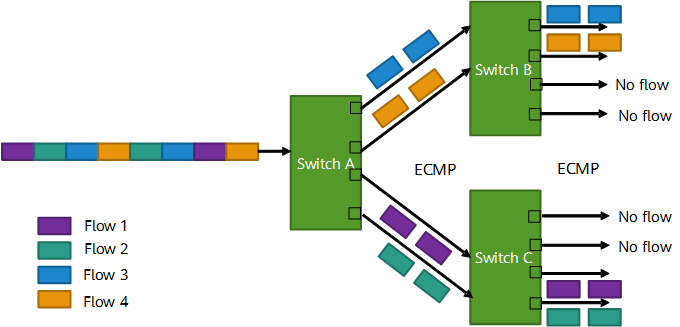
\includegraphics[width=\linewidth]{hash-polar.png}
  \caption{The Hash Polarization Issue}
  \label{fig:hash_polar}
\end{figure}

As we realize the first method has flaw that it depends on the implementation of the routers, as have designed a second structure. 
In this design, the routers can forward packets to multiple ports, but each forwarding contains a probability value. 
That is, a 2-way load balancer will send packets to both way with a "probability value" of 1/2. 
This allows use to analyze the amount of traffic through each equivlent router easily. 
However, this approach may not be able to verify the problem cause by internals of routers, like hash polarization. 
It is only verifying that there is no path that does not pass through even load balancing. 

\subsection{Optimization}\label{sec:opt}
The goal of optimization in code generation is to reduce unnecessary number of instructions, especially branches. Our optimization focuses on the common case of longest prefix matching based stateless routers without ACL or ECMP. There are two aspects of optimization we hope to achieve. Firstly, the routing table lookup has lots of branches and we hope to improve the performance by both compressing the routing table and using a efficient lookup algorithm. Secondly, a group of routers can be replaced as a single node with the same behavior from the outside point of view. This grouping of nodes and abstracting them as a single one allows joint optimization and lookup of all the FIBs in this group.

To achieve this goal, equivalence classes are first generated from forwarding tables of the selected group of nodes using atomic predicate. Then, a concrete packet of each equivalence class is injected to each the nodes in the group in the generated network simulator to find where packets of the equivalence class exits the group. Lastly, giving a set of <equivalence class, input node, output node, output port>, we generate a C++ Router class that forwards the packet by looking up a equivalence class based lookup table using binary search on ranges~\cite{binary_search_lookup}.

Figure~\ref{fig:opt} shows the implementation of the optimization procedure. Other than the network configuration, the user also provides a group of nodes to act as a "component" that will be optimized to a single node. Equivalence classes will be generated first using a bit trie with the idea of Atomic Predicate. For each of the equivalence class, a concrete packet is also generated. With these information, a network simulator will be generated that injects a concrete packet of each equivalence class to each node in the group. The execution of the simulator will record where each of these injected packet exit the group of nodes. The output is then used to generate a single node class that make forwarding decision by looking up the input equivalence class using binary search on ranges.

By merging consecutive ranges having the same forwarding result before generating code for binary search, the routing table can effectively be compressed.

\begin{figure}[]
 \centering
 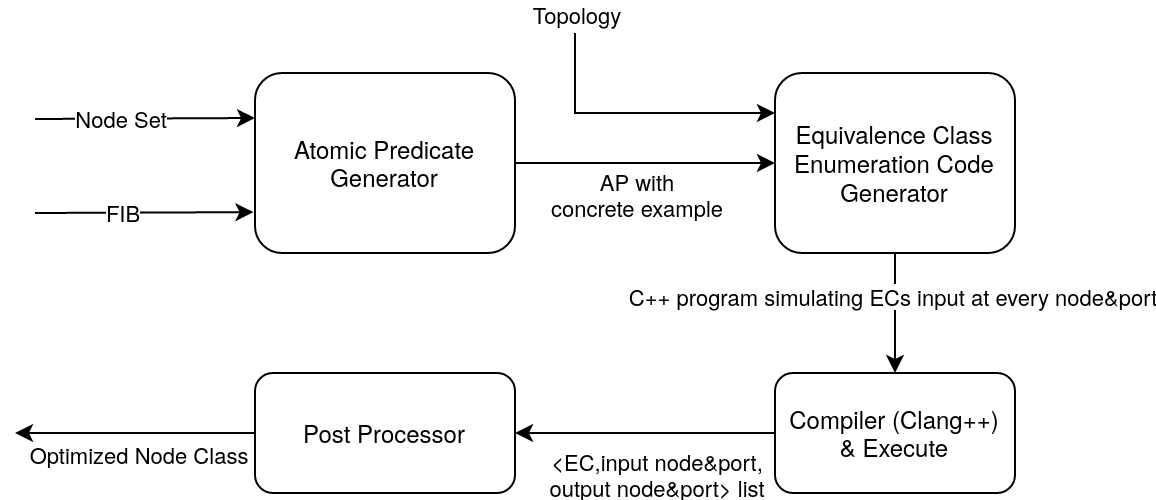
\includegraphics[width=\linewidth]{optimization.png}
 \caption{Optimization Implementation}
 \label{fig:opt}
\end{figure}

Listing~\ref{code:opt} shows a generated optimized router class. The nested if are the inlined binary search procedure.

\begin{lstlisting}[  language=C,
 caption=Optimization of Router: Binary Search on Ranges,
 label=code:opt,
 captionpos=b,
 basicstyle=\tiny]
class LeafP19S3 {
 public:
 PktState forward(PktState stateIn) { //generated-comment: [reached] LeafP19S3
  int node = stateIn.node;
  int portIn = stateIn.port;
  Header &header = stateIn.header;
  if (header.dst_address >= 0xa130600 && header.dst_address <= 0xa1306ff)
  return {header, 449, -1};
  else if (header.dst_address < 0xa130600) {
   if (header.dst_address >= 0xa130200 && header.dst_address <= 0xa1302ff)
   return {header, 445, -1};
   else if (header.dst_address < 0xa130200) {
    if (header.dst_address >= 0xa130000 && header.dst_address <= 0xa1300ff)
    return {header, 435, -1};
    else if (header.dst_address < 0xa130000) {
     return {header, 435, 12};
    } else {
     return {header, 432, -1};
    }
   } else {
    if (header.dst_address >= 0xa130400 && header.dst_address <= 0xa1304ff)
    return {header, 447, -1};
    else if (header.dst_address < 0xa130400) {
     return {header, 446, -1};
    } else {
     return {header, 448, -1};
    }
   }
  } else {
   if (header.dst_address >= 0xa130a00 && header.dst_address <= 0xa130aff)
   return {header, 453, -1};
   else if (header.dst_address < 0xa130a00) {
    if (header.dst_address >= 0xa130800 && header.dst_address <= 0xa1308ff)
    return {header, 451, -1};
    else if (header.dst_address < 0xa130800) {
     return {header, 450, -1};
    } else {
     return {header, 452, -1};
    }
   } else {
    if (header.dst_address >= 0xa130c00 && header.dst_address <= 0xa130cff)
    return {header, 455, -1};
    else if (header.dst_address < 0xa130c00) {
     return {header, 454, -1};
    } else {
     if (header.dst_address >= 0xa140000)
     return {header, 435, 12};
     return {header, 435, -1};
     
    }
   }
  }
  assert(0);
 }
};

\end{lstlisting}
\section{Evaluation}\label{sec:eval}

\section{FUTURE DIRECTION}\label{sec:fd}

\section{CONCLUSIONS}\label{sec:c}




\addtolength{\textheight}{-12cm}  
\bibliographystyle{IEEEtran}
\bibliography{bibs}


\end{document}

